\nsection{OSN 6 Основные понятия безопасности информации: конфиденциальность, целостность, доступность. Виды защиты информации. Модель Белла-Лападулы. Понятие ошибки, уязвимости в программном обеспечении, примеры.}

\textbf{Конфиденциальность} – это гарантия, что информация может быть прочитана и проинтерпретирована только теми людьми и процессами, которые авторизованы это делать. Обеспечение конфиденциальности включает процедуры и меры, предотвращающие раскрытие информации неавторизованными пользователями. \textbf{Примером} может являться почтовое сообщение, которое защищено от прочтения кем бы то ни было, кроме адресата.

\textbf{Целостность} – это гарантирование того, что информация остается неизменной, корректной и аутентичной. Обеспечение целостности предполагает предотвращение и определение неавторизованного создания, модификации или удаления информации. \textbf{Примером} могут являться меры, гарантирующие, что почтовое сообщение не было изменено при пересылке.

\textbf{Доступность} – это гарантирование того, что авторизованные пользователи могут иметь доступ и работать с информационными активами, ресурсами и системами, которые им необходимы, при этом обеспечивается требуемая производительность. Обеспечение доступности включает меры для поддержания доступности информации, несмотря на возможность создания помех, включая отказ системы и преднамеренные попытки нарушения доступности. \textbf{Примером} может являться защита доступа и обеспечение пропускной способности почтового сервиса.

\textbf{Еще примеры}:
\begin{itemize}
    \item Нарушение конфиденциальности:
        \begin{itemize}
            \item OpenSSL Heartbleed;
            \item программная закладка в роутере;
            \item шпионаж через веб-камеру в телевизоре.
        \end{itemize}
    \item Нарушение целостности:
        \begin{itemize}
            \item программная закладка в роутере;
            \item изменение базы данных с паролями через внедрение
SQL-кода.
        \end{itemize}
    \item Нарушение доступности:
    \begin{itemize}
        \item аварийное завершение программы;
        \item отказ в обслуживании - DoS, DDoS.
    \end{itemize}
\end{itemize}

\textbf{Защита информации} – это деятельность, направленная на предотвращение утечки защищаемой информации, несанкционированных и непреднамеренных воздействий. Такая деятельность может быть: 1) \textbf{правовой}, регулирующей защиту информации путем разработки правовых норм и документов, а также надзор и контроль над их исполнением; 2) \textbf{технической} – путем использования программного обеспечения; 3) \textbf{криптографической} – путем преобразования информации; 4) \textbf{физической} – посредством организационных мероприятий, препятствующих доступу к конфиденциальной информации

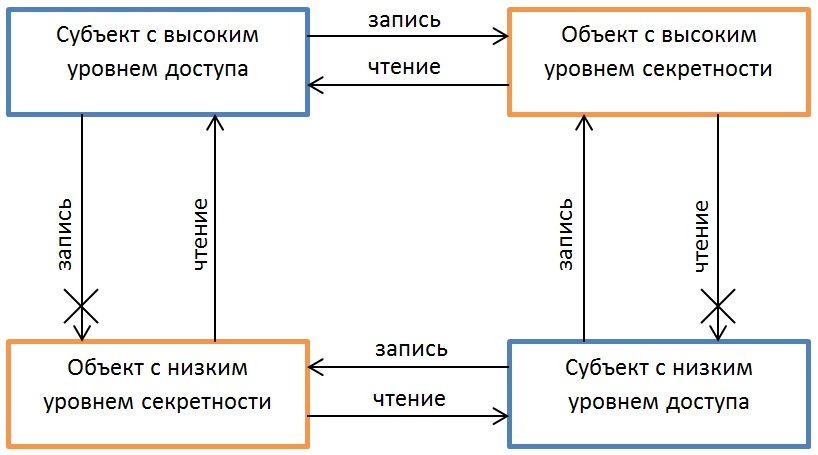
\includegraphics[scale=0.4]{pics/bella.png}

\textbf{Модель Белла — Лападулы} — модель контроля и управления доступом, основанная на мандатной модели управления доступом. В модели анализируются условия, при которых невозможно создание информационных потоков от субъектов с более высоким уровнем доступа к субъектам с более низким уровнем доступа. Модель Белла — Лападулы является моделью разграничения доступа к защищаемой информации. Все элементы, входящие в состав информационной системы, разделены на две категории — \textbf{субъекты и объекты}. Каждому субъекту присваивается свой \textbf{уровень доступа}, соответствующий степени конфиденциальности. Аналогично, объекту присваивается \textbf{уровень секретности}. \textbf{Понятие защищённой системы} определяется следующим образом: каждое состояние системы должно соответствовать политике безопасности, установленной для данной информационной системы. Переход между состояниями описывается функциями перехода. Система находится в безопасном состоянии в том случае, если у каждого субъекта имеется доступ только к тем объектам, к которым разрешен доступ на основе текущей политики безопасности. Для определения, имеет ли субъект права на получение определенного вида доступа к объекту, уровень секретности субъекта сравнивается с уровнем секретности объекта, и на основе этого сравнения решается вопрос, предоставить или нет запрашиваемый доступ. \textbf{Наборы уровень доступа/уровень секретности описываются с помощью матрицы доступа.}

\textbf{Ошибки в программах:}
\textbf{Ошибки в логике приложения}, \textbf{Ошибки уровня архитектуры приложения}
(неверная работа с разделяемыми ресурсами в многопоточном ПО), \textbf{Несоответствие модели языка программирования}
(выход за границы массива, нарушение правил алиасинга, ABI),\textbf{ Несоответствие требованиям со стороны аппаратуры}
(неверная адресация в памяти, целочисленное деление на 0).

В компьютерной безопасности термин \textbf{«уязвимость»}(англ. vulnerability) используется для обозначения недостатка в системе, используя который, можно намеренно нарушить её целостность и вызвать неправильную работу. 

\textbf{Уязвимость информационной системы} —
свойство информационной системы,
обусловливающее возможность
реализации угроз безопасности
обрабатываемой в ней информации.

\textbf{Угроза безопасности информации} —
совокупность условий и факторов,
создающих потенциальную или реально
существующую опасность нарушения
безопасности информации.

Уязвимость может быть результатом ошибок программирования, недостатков, допущенных при проектировании системы, ненадежных паролей, вирусов и других вредоносных программ, скриптовых и SQL-инъекций. Некоторые уязвимости известны только теоретически, другие же активно используются и имеют известные \textbf{эксплойты}.

Обычно уязвимость позволяет атакующему «обмануть» приложение — заставить его совершить действие, на которое у того не должно быть прав. Это делается путём внедрения каким-либо образом в программу данных или кода в такие места, что программа воспримет их как «свои». Некоторые уязвимости появляются из-за недостаточной проверки данных, вводимых пользователем, и позволяют вставить в интерпретируемый код произвольные команды (SQL-инъекция, XSS, SiXSS). Другие уязвимости появляются из-за более сложных проблем, таких как запись данных в буфер без проверки его границ (переполнение буфера).

\textbf{Эксплоит} — программа, фрагмент кода или последовательность команд, использующие уязвимость, чтобы добиться непредусмотренного поведения информационной системы.
В идеале атакующий пытается перехватить поток управления уязвимой системы, чтобы выполнить произвольный код:
\begin{itemize}
    \item полезная нагрузка — внедряемый код;
    \item шелл-код — полезная нагрузка, дающая доступ к интерпретатору команд ОС.
\end{itemize}